\documentclass{../../../oss-ap12ibhl}
%\pgfplotsset{compat=1.16}
%
\begin{document}
\genheader

\gentitle{6}{ROTATIONAL MOTION}

\begin{questions}

  \question What defines a lever arm?
  \begin{choices}
    \choice The distance parallel to the line of action of the force
    \choice The distance parallel to the line of action of the force from the
    pivot point
    \choice The length of the lever
    \choice The perpendicular distance from the pivot to the line of action of
    the force
    \choice $F = |F|cos(\theta)x$
  \end{choices}
    
  \question The most general statement of Newton's first law is:
  \begin{choices}
    \choice $\sum\bm{F}=\bm{0}$
    \choice $\sum F_x=0$, $\sum F_y=0$ and $\sum F_z=0$
    \choice All the forces or moments must be zero.
    \choice All the forces added together must be zero.
    \choice $\sum F_x=0$, $\sum F_y=0$ and $\sum F_z=0$, $\sum\tau_x=0$,
    $\sum\tau_y=0$ and $\sum\tau_z=0$,
  \end{choices}

  \question When a skater performs a spin on ice with his arms outstretched,
  what happens when he brings his arms close to his body?
  \begin{choices}
    \choice His angular acceleration decreases because his moment of inertia
    was decreased.
    \choice His angular acceleration increases because his moment of inertia
    was decreased.
    \choice His angular velocity decreases because his moment of inertia was
    decreased.
    \choice His angular velocity increases because his moment of inertia was
    decreased.
    \choice His angular displacement increases because his moment of inertia
    was decreased
  \end{choices}
  \vspace{.7in}
    
  \question Linear acceleration is to force as angular acceleration is to
  \begin{choices}
    \choice kinetic energy
    \choice angular velocity
    \choice rotational inertia
    \choice torque
    \choice angular momentum
  \end{choices}

  \question A meter stick of mass \SI{.1}{\kilo\gram} rests on a table as
  shown. A length of \SI{40}{\centi\metre} extends over the edge of the table.
  How far from the edge of the table could a \SI{.05}{\kilo\gram} mass be
  placed on the meter stick so that the stick just begins to tip?

  \begin{minipage}{.35\linewidth}
    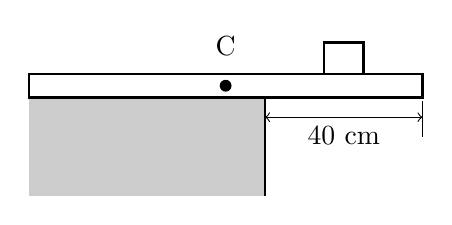
\begin{tikzpicture}[scale=5]
      \fill[gray!40](0,-.25) rectangle(.6,0);
      \begin{scope}[thick]
        \draw(0,0) rectangle(1,.06);
        \draw(.6,0)--(.6,-.25);
        \draw(.75,.06) rectangle (.85,.14);
      \end{scope}
      \draw(1,-.01)--(1,-.1);
      \draw[<->](.6,-.05)--(1,-.05) node[midway,below]{40 cm};
      \fill(.5,.03) circle(.015);
      \node at (.5,.13){C};
    \end{tikzpicture}
  \end{minipage}
  \begin{minipage}{.4\linewidth}  
    \begin{choices}
      \choice\SI{5}{\centi\metre}
      \choice\SI{10}{\centi\metre}
      \choice\SI{15}{\centi\metre}
      \choice\SI{20}{\centi\metre}
      \choice\SI{30}{\centi\metre}
    \end{choices}
  \end{minipage}
%    \columnbreak

  \question The moment of inertia of a particular thin-walled cylinder around
  its central axis is given by $mR^2$. What expression best represents the
  angular momentum of this cylinder if it spins about the central axis at a
  rate of 12 revolutions per second?
  \begin{choices}
    \choice $24\pi mR^2$
    \choice $12\pi mR^2$
    \choice $12mR^2$
    \choice $\dfrac1{12}\pi mR^2$
    \choice $\dfrac1{12\pi}mR^2$
  \end{choices}
    
  \question A meter stick is balanced on a fulcrum at its center, as shown. A
  mass of \SI{5}{\kilo\gram} is hung on the left end of the stick, and a mass of
  \SI{2}{\kilo\gram} is hung on the right end. In order to balance the
  system, a mass $m$ is hung at the 25-cm mark on the right
  side. What is the value of the mass $m$?

  \vspace{.1in}
  \begin{minipage}{.5\linewidth}
    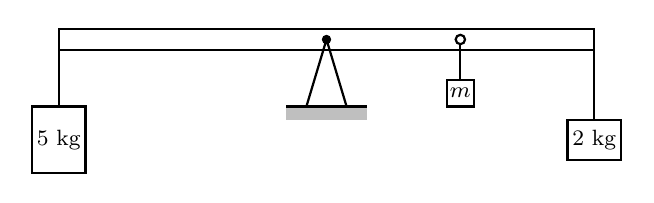
\begin{tikzpicture}[scale=1.7]
      \begin{scope}[thick]
        \draw(-2,-.08) rectangle(2,.08);
        \fill(0,0) circle(.035);
        \draw(-2,0)--(-2,-.5);
        \draw(2,0)--(2,-.6);
        \draw(-2.2,-.5) rectangle(-1.8,-1) node[midway]{\footnotesize 5 kg};
        \draw(2.2,-.6) rectangle(1.8,-.9) node[midway]{\footnotesize 2 kg};
        \draw(1,0) circle(.035);
        \draw(1,-.035)--(1,-.3);
        \draw(.9,-.3) rectangle(1.1,-.5) node[midway]{\footnotesize$m$};
        \fill[gray!50](-.3,-.6) rectangle(.3,-.5);
        \draw(0,0)--(-.15,-.5)--(.15,-.5)--cycle;
        \draw(-.3,-.5)--(.3,-.5);
      \end{scope}
    \end{tikzpicture}
  \end{minipage}
  \begin{minipage}{.2\linewidth}
    \begin{choices}
      \choice\SI{12}{\kilo\gram}
      \choice\SI6{\kilo\gram}
      \choice\SI4{\kilo\gram}
      \choice\SI3{\kilo\gram}
      \choice\SI2{\kilo\gram}
    \end{choices}
  \end{minipage}
  
  \question A metal bar of constant density and weight $W$ is attached to a
  pivot on the wall at point $P$ and supported by a rope that makes an angle of
  \ang{60} with the vertical wall. The reaction force exerted by the pivot on
  the bar at point $P$ is best represented by which arrow?

  \begin{minipage}{.3\linewidth}
    \pic{.85}{metal-bar}
  \end{minipage}
  \begin{minipage}{.3\linewidth}
    \begin{choices}
      \choice{\Huge $\nearrow$}
      \choice{\Huge $\uparrow$}
      \choice{\Huge $\downarrow$}
      \choice{\Huge $\nwarrow$}
      \choice{\Huge $\searrow$}
    \end{choices}
  \end{minipage}
  \newpage
  
  \question A uniform rod of length $L$ and mass $m$ has a rotational inertia of
  $\displaystyle \frac1{12}mL^2$ about its center. A particle, also of mass
  $m$, is attached to one end of the stick. The combined rotational inertia of
  the stick and particle about the center of the rod is

  \begin{minipage}{.4\linewidth}
    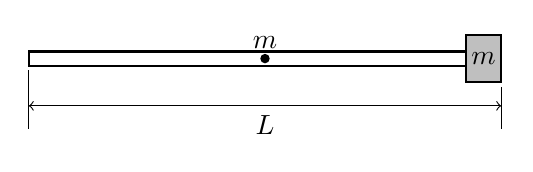
\begin{tikzpicture}[scale=3]
      \draw[thick](-1,-.03) rectangle (1,.03);
      \fill(0,0) circle(.02) node[above]{$m$};
      \draw[thick,fill=gray!50](.85,-.1) rectangle(1,.1) node[midway]{$m$};
      \draw[<->](-1,-.2)--(1,-.2) node[midway,below]{$L$};
      \draw(-1,-.05)--(-1,-.3);
      \draw(1,-.12)--(1,-.3);
    \end{tikzpicture}
  \end{minipage}
  \begin{minipage}{.2\linewidth}
    \begin{choices}
      \choice$\dfrac{mL^2}{3}$
      \choice$\dfrac{12mL^2}{13}$
      \choice$\dfrac{13mL^2}{12}$
      \choice$\dfrac{mL^2}{156}$
      \choice$\dfrac{13mL^2}{156}$
    \end{choices}
  \end{minipage}
%    \columnbreak

  \question A hoop of radius $R$ and mass $m$ has a rotational inertia of
  $mR^2$. The hoop rolls without slipping along a horizontal floor with a
  constant speed $v$ and then rolls up a long incline. The hoop can roll up the
  incline to a maximum vertical height of

  \begin{minipage}{.5\linewidth}
    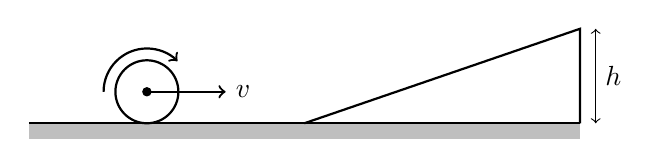
\begin{tikzpicture}
      \fill[gray!50](0,-.2) rectangle(7,0);
      \begin{scope}[thick]
        \draw(0,0)--(7,0);
        \draw(3.5,0)--(7,1.2)--(7,0);
        \draw(1.5,.4) circle(.4);
        \fill(1.5,.4) circle(.06);
        \draw[->](1.5,.4)--(2.5,.4) node[right]{$v$};
        \draw[->](.95,.4) arc(180:45:.55);
      \end{scope}
      \draw[<->](7.2,0)--(7.2,1.2) node[midway,right]{$h$};
    \end{tikzpicture}
  \end{minipage}
  \begin{minipage}{.2\linewidth}
    \begin{choices}
      \choice$\dfrac{v^2}{g}$
      \choice$\dfrac{2v^2}{g}$
      \choice$\dfrac{v^2}{2g}$
      \choice$\dfrac{4v^2}{g}$
      \choice$\dfrac{v^2}{4g}$
    \end{choices}
  \end{minipage}
    
  \question Two disks are fixed to a vertical axle that is rotating with a
  constant angular speed $\omega$. The smaller disk has a mass $m$ and a radius
  $r$, and the larger disk has a mass $2m$ and radius $2r$. The general equation
  for the rotational inertia of a disk of mass $M$ and radius $R$ is
  $\frac12MR^2$. The ratio of the angular momentum of the larger disk to
  the smaller disk is

  \begin{minipage}{.35\linewidth}
    \cpic{.85}{2disks}
    \end{minipage}
  \begin{minipage}{.3\linewidth}
    \begin{choices}
      \choice $1:4$
      \choice $4:1$
      \choice $1:2$
      \choice $2:1$
      \choice $8:1$
    \end{choices}
  \end{minipage}
  
  \question A light rod has a mass attached at each end. At one end is a
  \SI{6}{\kilo\gram} mass, and at the other end is a \SI{3}{\kilo\gram} mass.
  An axis can be placed at any of the points shown. Through which point should
  an axis be placed so that the rotational inertia is the greatest about that
  axis?
  \begin{center}
    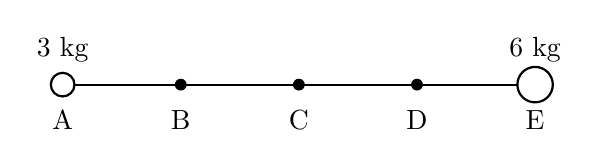
\begin{tikzpicture}[scale=1.5]
      \begin{scope}[thick]
        \draw(0,0) circle(.1);
        \draw(4,0) circle(.15);
        \draw(.1,0)--(3.85,0);
      \end{scope}
      \fill (1,0) circle(.05);
      \fill (2,0) circle(.05);
      \fill (3,0) circle(.05);
      \node at (0,-.3){A};
      \node at (1,-.3){B};
      \node at (2,-.3){C};
      \node at (3,-.3){D};
      \node at (4,-.3){E};
      \node at (0,.3){3 kg};
      \node at (4,.3){6 kg};
    \end{tikzpicture}
  \end{center}
  \begin{oneparchoices}
    \choice A\hspace{.4in}
    \choice B\hspace{.4in}
    \choice C\hspace{.4in}
    \choice D\hspace{.4in}
    \choice E
  \end{oneparchoices}
  \vspace{.2in}
    
  \question Astronauts are conducting an experiment in a negligible gravity
  environment. Two spheres of mass $m$ are attached to either end of a light
  rod. As the rod and spheres float motionless in space, an astronaut launches
  a piece of sticky clay, also of mass $m$, toward one of the spheres so that
  the clay strikes and sticks to the sphere perpendicular to the rod. Which of
  the following statements is true of the motion of the rod, clay, and spheres
  after the collision?

  \begin{minipage}{.3\linewidth}
    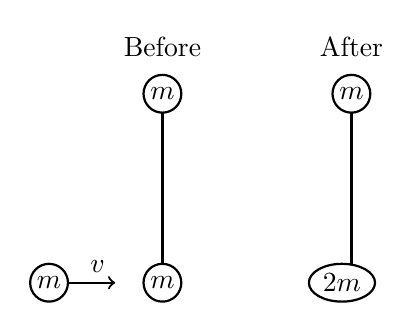
\begin{tikzpicture}[scale=1.2]
      \begin{scope}[thick]
        \draw(0,0) circle(.2) node{$m$};
        \draw(0,2) circle(.2) node{$m$};
        \draw(0,.2)--(0,1.8);
        \draw(-1.2,0) circle(.2) node{$m$};
        \draw[->](-1,0)--(-.5,0) node[above left]{$v$};
        
        \draw(1.9,0) ellipse(.35 and .2) node{$2m$};
        \draw(2,2) circle(.2) node{$m$};
        \draw(2,.2)--(2,1.8);
      \end{scope}
      \node at (0,2.5) {Before};
      \node at (2,2.5) {After};
    \end{tikzpicture}
  \end{minipage}
  \begin{minipage}{.69\linewidth}
    \begin{choices}
      \choice Linear momentum is not conserved, but angular momentum is
      conserved.
      \choice Angular momentum is not conserved, but linear momentum is
      conserved.
      \choice Kinetic energy is conserved, but angular momentum is not
      conserved.
      \choice Kinetic energy is conserved, but linear momentum is not
      conserved.
      \choice Both linear momentum and angular momentum are conserved, but
      kinetic energy is not conserved.
    \end{choices}
  \end{minipage}
  \vspace{.7in}
    
  \question A cylinder has a moment of inertia, $I$. How much time does it take
  a torque, $\tau$, to increase its angular speed from $\omega_1$ to $\omega_2$?
  \begin{choices}
    \choice $\dfrac{I(\omega_2-\omega_1)}{\tau}$
    \choice $\dfrac{\tau}{I(\omega_2-\omega_1)}$
    \choice $I(\omega_2-\omega_1)\tau$
    \choice $\dfrac{2\tau}{I(\omega_2^2-\omega_1^2)}$
    \choice $\dfrac12I(\omega_2^2-\omega_1^2)\tau$
  \end{choices}
  \newpage
  
  \question One end of a stick of length $L$, rotational inertia $I$, and mass
  $m$ is pivoted on an axle with negligible friction at point $P$. The other end
  is tied to a string and held in a horizontal position. When the string is
  cut, the stick rotates counterclockwise. The angular speed $\omega$ of the
  stick when it reaches the bottom of its swing is

  \begin{minipage}{.45\linewidth}
    \pic{.82}{end-of-stick}
  \end{minipage}
  \begin{minipage}{.4\linewidth}
    \begin{choices}
    \choice$\dfrac{mgL}{I}$
    \choice$\sqrt{\dfrac{mgL}{I}}$
    \choice$\sqrt{\dfrac{2mgL}{I}}$
    \choice$\sqrt{\dfrac{mgL}{2I}}$
    \choice$\sqrt{\dfrac{4mgL}{I}}$
    \end{choices}
  \end{minipage}
    
  \question A disk is mounted on a fixed axle. The rotational inertia of the
  disk is $I$. The angular velocity of the disk is decreased from $\omega_0$ to
  $\omega_f$ during a time $\Delta t$ due to friction in the axle. The
  magnitude of the average net torque acting on the wheel is
  \begin{choices}
    \choice $\dfrac{\omega_f-\omega_0}{\Delta t}$
    \choice $\dfrac{(\omega_f-\omega_o)^2}{\Delta t}$
    \choice $\dfrac{I(\omega_f-\omega_o)}{\Delta t}$
    \choice $\dfrac{I(\omega_f-\omega_o)^2}{\Delta t}$
    \choice $\dfrac{I(\omega_f-\omega_o)}{\Delta t^2}$
  \end{choices}
    
  \question The average power developed by the friction in the axle of the disk
  from the previous question to bring it to a complete stop is
  \begin{choices}
    \choice $\dfrac{\omega_0}{\Delta t}$
    \choice $\dfrac{(\omega_0)^2}{\Delta t}$
    \choice $\dfrac{I\omega_0}{2\Delta t}$
    \choice $\dfrac{I\omega_0^2}{2\Delta t}$
    \choice $\dfrac{I(\omega_f-\omega_0)}{\Delta t^2}$
  \end{choices}

  \uplevel{
    \textbf{Question \ref{lightrod1}--\ref{lightrod2}}

    A light rod of negligible mass is pivoted at point $P$ a distance $L$ from
    one end as shown. A mass $m$ is attached to the left end of the rod at
    a distance of $3L$ from the pivot, and another mass $4m$ is attached to the
    other end a distance $L$ from the pivot. The system begins from rest in the
    horizontal position.
    \begin{center}
      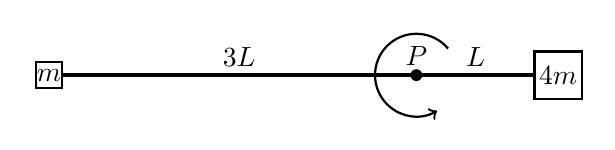
\begin{tikzpicture}[scale=1.5]
        \draw[very thick](-3,0)--(1,0);
        \draw[thick](1,-.2) rectangle(1.4,.2) node[midway]{$4m$};
        \draw[thick](-3,-.11) rectangle(-3.22,.11) node[midway]{$m$};
        \fill(0,0) circle(.05) node[above]{$P$};
        \node at (.5,.15){$L$};
        \node at (-1.5,.15){$3L$};
        \draw[thick,->,rotate=40](.35,0) arc(0:260:.35);
      \end{tikzpicture}
    \end{center}
  }


  \question The net torque acting on the system due to gravitational forces is
  \label{lightrod1}
  \begin{choices}
    \choice $4mgL$ clockwise
    \choice $3mgL$ clockwise
    \choice $3mgL$ counterclockwise
    \choice $mgL$ counterclockwise
    \choice $mgL$ clockwise
  \end{choices}
    
  \question The angular acceleration of the system when it is released from
  rest is
  \begin{choices}
    \choice zero
    \choice $\dfrac{g}{5L}$
    \choice $\dfrac{g}{4L}$
    \choice $\dfrac{g}{13L}$
    \choice $\dfrac{g}{L}$
  \end{choices}
  \label{lightrod2}
  \newpage
  
  % TAKEN FROM THE 2016 AP PHYSICS 1 EXAM FREE-RESPONSE QUESTION #1
  \uplevel{
    \cpic{.4}{wooden-wheel1}
  }

  \question A wooden wheel of mass $M$, consisting of a rim with spokes, rolls
  down a ramp that makes an angle $\theta$ with the horizontal, as shown above.
  The ramp exerts a force of static friction on the wheel so that the wheel
  rolls without slipping.
  \begin{parts}
  \part
    \begin{subparts}
      \subpart On the diagram below, draw and label the forces (not components)
      that act on the wheel as it rolls down the ramp, which is indicated by the
      dashed line. To clearly indicate at which point on the wheel each force
      is exerted, draw each force as a distinct arrow starting on, and pointing
      away from, the point at which the force is exerted. The lengths of the
      arrows need not indicate the relative magnitudes of the forces.
      \cpic{.22}{wooden-wheel2}
      
      \subpart As the wheel rolls down the ramp, which force causes a change in
      the angular velocity of the wheel with respect to its center of mass?
      Briefly explain your reasoning.
    \end{subparts}

    \part For this ramp angle, the force of friction exerted on the wheel is
    less than the maximum possible static friction force. Instead, the
    magnitude of the force of static friction exerted on the wheel is 40
    percent of the magnitude of the force or force component directed opposite
    to the force of friction. Derive an expression for the linear acceleration
    of the wheel's center of mass in terms of $M$, $\theta$, and physical
    constants, as appropriate.
    
    \part In a second experiment on the same ramp, a block of ice, also with
    mass $M$, is released from rest at the same instant the wheel is released
    from rest, and from the same height. The block slides down the ramp with
    negligible friction.
    \begin{subparts}
      \subpart Which object, if either, reaches the bottom of the ramp with the
      greatest speed?Briefly explain your answer, reasoning in terms of forces.

      \vspace{.1in}
      \underline{\hspace{.3in}} Wheel\hspace{.2in}
      \underline{\hspace{.3in}} Block\hspace{.2in}
      \underline{\hspace{.3in}} Neither; both reach the bottom with the same
      speed.

      \subpart Briefly explain your answer again, now reasoning in terms of
      energy.
    \end{subparts}
  \end{parts}
  \newpage
  
  % TAKEN FROM THE 2018 AP PHYSICS 1 EXAM FREE-RESPONSE QUESTION #1
  \uplevel{
    \begin{center}
      \pic{.4}{spacecraft1}
      
      \underline{Note:} Figure not drawn to scale.
    \end{center}
  }
  \question A spacecraft of mass $m$ is in a clockwise circular orbit of radius
  $R$ around Earth, as shown in the figure above. The mass of Earth is $M_E$.
  \begin{parts}
    \part In the figure below, draw and label the forces (not components) that
    act on the spacecraft. Each force must be represented by a distinct arrow
    starting on, and pointing away from, the spacecraft.

    \uplevel{
      \begin{center}
        \pic{.3}{spacecraft2}
        
        \underline{Note:} Figure not drawn to scale.
      \end{center}
    }
    
  \part
    \begin{subparts}
      \subpart Derive an equation for the orbital period $T$ of the spacecraft
      in terms of $m$, $M_E$, $R$, and physical constants, as appropriate. If
      you need to draw anything other than what you have shown in part (a) to
      assist in your solution, use the space below. Do NOT add anything to the
      figure in part (a).

      \subpart A second spacecraft of mass $2m$ is placed in a circular orbit
      with the same radius $R$. Is the orbital period of the second spacecraft
      greater than, less than, or equal to the orbital period of the first
      spacecraft? Briefly explain your reasoning.

      \vspace{.1in}
      \underline{\hspace{.3in}}Greater than\hspace{.2in}
      \underline{\hspace{.3in}}Less than\hspace{.2in}
      \underline{\hspace{.3in}}Equal to
    \end{subparts}
    
    \part The first spacecraft is moved into a new circular orbit that has a
    radius greater than $R$, as shown in the figure below.

    \uplevel{
      \begin{center}
        \pic{.3}{spacecraft3}

        \underline{Note:} Figure not drawn to scale.
      \end{center}
    }
    Is the speed of the spacecraft in the new orbit greater than, less than, or
    equal to the original speed? Briefly explain your reasoning.
    
    \vspace{.1in}
    \underline{\hspace{.3in}}Greater than\hspace{.2in}
    \underline{\hspace{.3in}}Less than\hspace{.2in}
    \underline{\hspace{.3in}}Equal to
  \end{parts}
  \newpage

  \uplevel{
    \cpic{.35}{disk1}
  }
  \question The disk shown above spins about the axle at its center. A student's
  experiments reveal that, while the disk is spinning, friction between the
  axle and the disk exerts a constant torque on the disk.
  \begin{parts}
    \part At time $t=0$ the disk has an initial counterclockwise (positive)
    angular velocity $\omega_0$. The disk later comes to rest at time $t=t_1$.
    \begin{subparts}
      \subpart On the grid at left below, sketch a graph that could represent
      the disk's angular velocity as a function of time $t$ from $t=0$ until the
      disk comes to rest at time $t=t_1$.
      
      \subpart On the grid at right below, sketch the disk's angular
      acceleration as a function of time $t$ from $t=0$ until the disk comes to
      rest at time $t=t_1$.   
    \end{subparts}

    \uplevel{
      \cpic{.9}{graph1}
    }
    
    \part The magnitude of the frictional torque exerted on the disk is
    $\tau_0$ . Derive an equation for the rotational inertia $I$ of the disk in
    terms of $\tau_0$, $\omega_0$, $t_1$, and physical constants, as
    appropriate.
    \newpage
    
    \part In another experiment, the disk again has an initial positive angular
    velocity $\omega_0$ at time $t=0$. At $t=\dfrac12t_1$, the student starts
    dripping oil on the contact surface between the axle and the disk to reduce
    the friction. As time passes, more and more oil reaches that contact
    surface, reducing the friction even further.
    \begin{subparts}
      \subpart On the grid at left below, sketch a graph that could represent
      the disk's angular velocity as a function of time from $t=0$ to $t=t_1$,
      which is the time at which the disk came to rest in part (a).

      \subpart On the grid at right below, sketch the disk's angular
      acceleration as a function of time from $t=0$ to $t=t_1$.
    \end{subparts}

    \uplevel{
      \cpic{.9}{graph2}
    }
    
    \part The student is trying to mathematically model the magnitude $\tau$ of
     the torque exerted by the axle on the disk when the oil is present at
     times $t>\dfrac12t_1$. The student writes down the following two
     equations, each of which includes a positive constant ($C_1$ or $C_2$)
     with appropriate units.
     \begin{enumerate}
       \item $\tau=C_1\left(t-\dfrac12t_1\right)$ (for $t>\dfrac12 t_1$)
       \item $\tau=\dfrac{C_2}{\left(t+\dfrac12t_1\right)}$ (for
         $t>\dfrac12t_1$)
     \end{enumerate}
     Which equation better mathematically models this experiment? Briefly
     explain why the equation you selected is plausible and why the other
     equation is not plausible.

     \vspace{.1in}
     \underline{\hspace{.3in}}Equation (1)\hspace{.2in}
     \underline{\hspace{.3in}}Equation (2)
  \end{parts}
\end{questions}
\end{document}
